\chapter{Технологический раздел}%
\label{cha:tekhnologicheskii_razdel}

\section{Выбор языка программирования и среды разработки}%
\label{sec:vybor_iazyka_programmirovaniia_i_sredy_razrabotki}

Разработанный модуль ядра написан на языке программирования C. Выбор языка программирования С основан на том, что исходный код
ядра Linux, все его модули и драйверы написаны на данном языке.
В качестве компилятора выбран gcc.

Для перехвата функций ядра была выбрана фреймворк ftrace.

\section{Некоторые моменты реализации}%
\label{sec:nekotorye_momenty_realizatsii}

При загрузке модуля производиться изменение указатель с исходных функций на собственные функции в таблице системных вызовов, и так начинает работу с пользовательским пространством.

При чтение из /proc/net/tcp tcp4\_seq\_show() будет вызываться повторно, и что во втором аргументе ему передается указатель на структуру sock. Единственное предостережение заключается в том, что иногда v не инициализируется (например, если просто печатается верхнюю строку таблицы). В данном случае v = 0x1, поэтому нужно проверить, что это не так, прежде чем пытаться разыменовать его.

Структура linux\_dirent64 - это то, что содержит информацию о списках каталогов (dirent - сокращение от “запись в каталоге”). определение можно найти в include/linux/dirent.h~\ref{lst:dirent}.

\begin{lstlisting}[language=c,caption={структура linux\_dirent64}, label=lst:dirent]
struct linux_dirent64 {
    u64         d_ino;
    s64         d_off;
    unsigned short      d_reclen;
    unsigned char       d_type;
    char        d_name[];
};
\end{lstlisting}

d\_reclen и d\_name. Первый - это длина записи и общий размер структуры в байтах. Это полезно, потому что позволяет нам легко перемещаться по этим структурам в памяти в поисках того, что нам нужно. В моем случае сравниваю d\_name с "." (текущий) и ".." (предыдущий), чтобы решить, какие записи следует скрыть. Оглядываясь назад на include/linux/readdir.c, видно, что d\_reclen используется именно таким образом (хотя и после того, как сначала был скопирован в другую структуру).

Функции для перехвата tcp4\_seq\_show, tcp6\_seq\_show, udp4\_seq\_show, udp6\_seq\_show, getdents64 определены в листинге~\ref{lst:defsh}.

\section{Апробация}%
\label{sec:aprobatsiia}

Рассмотрим примеры работы.

На рисунке~\ref{img:module_hide} демонстрируется сборка модуля, его загрузка, проверка скрытия и выгрузка.
\begin{figure}[H]
    \centering
    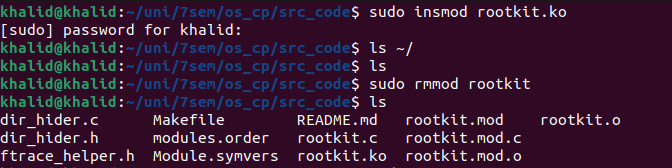
\includegraphics[scale=0.4]{img/file_and_directory.jpg}
    \caption{Загрузка, скрытие и выгрузка модуля}\label{img:module_hide}
\end{figure}

На рисунке~\ref{img:net_hide} демонстрируется скрытие сетевых сокетов.
\begin{figure}[H]
    \centering
    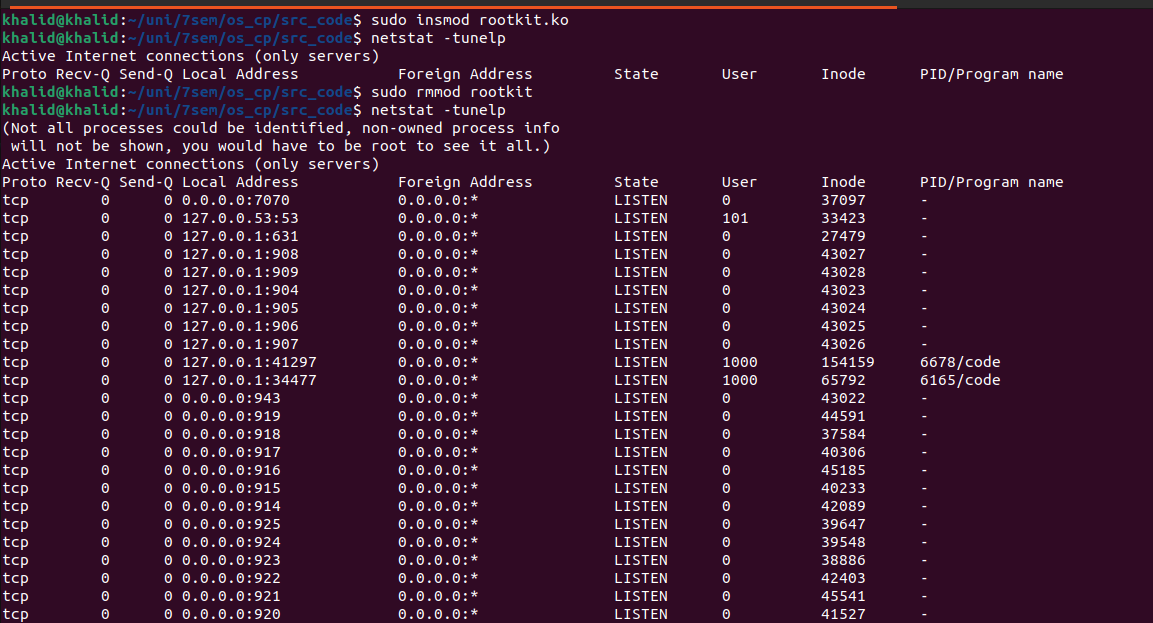
\includegraphics[scale=0.65]{img/net_sockets.jpg}
    \caption{Скрытие процесса}\label{img:net_hide}
\end{figure}

В ходе тестирования данного ПО не было выявлено ошибок.

\section*{Выводы}%
\label{sec:vyvody}

В данном разделе был обоснован выбор языка программирования, рассмотрены листинги реализованного программного обеспечения и приведены результаты работы ПО.

%%% mode: latex
%%% TeX-master: "rpz"
%%% End:
